\documentclass[../DS04.tex]{subfiles}
\graphicspath{{./figures/}}

\begin{document}

\prblm[40]{Cinétique de \ce{CaCO3}~: dissolution du calcaire et coraux}
% \subimport{/home/nora/Documents/Enseignement/Prepa/bpep/exercices/DS/cinetique_calcium/}{sujet.tex}
\subsection{Introduction}
\enonce{
  \paragraph*{Le calcium.}%
  Le calcium est le cinquième élément le plus abondant de la croûte terrestre.
  On le trouve dans les roches calcaires constituées principalement de carbonate
  de calcium \ce{CaCO3}. Le calcium joue un rôle essentiel chez la plupart des
  organismes vivants vertébrés en contribuant notamment à la formation des os
  ou des dents…
  \par
  Le calcium a également de nombreuses applications dans l’industrie en tant
  que réducteur des fluorures d’uranium notamment, de désoxydant pour différents
  alliages ferreux et non-ferreux, de désulfurant des hydrocarbures. Dans la
  métallurgie du plomb, les alliages calcium-magnésium sont utilisés afin
  d’éliminer les impuretés de bismuth.
  \par
  Les coraux sont généralement des colonies de polypes qui vivent regroupées
  pour former des superorganismes partageant un squelette calcaire. Les coraux
  durs, «~constructeurs de récifs~», ont formé par accumulation de ces
  squelettes minéraux des récifs coralliens dont certains sont devenus les plus
  grandes structures complexes connues créées par des organismes vivants (les
  grandes barrières de corail).

  \paragraph*{Potentiel hydrogène pH.}%
  On rappelle la définition du pH~:
    \[
      \pH = -\log [\ce{H+}]
    \]
  où $\log$ est le logarithme en base $10$ et $[\ce{H+}]$ est la
  concentration d'ion oxonium en $\si{mol.L^{-1}}$.

  \paragraph*{Réaction de dissolution.}%
  On s’intéresse maintenant à la vitesse de la réaction de dissolution du
  carbonate de calcium selon deux méthodes. Pour cela, on étudie l’évolution de
  la réaction entre le carbonate de calcium \ce{CaCO3(s)} et un volume $V_0 =
  \SI{100}{\milli\litre}$ d’une solution d’acide chlorhydrique de concentration
  $c_a = \SI{0,10}{\mol\per\litre}$. L’équation de la réaction s’écrit~:
  \[
        \ce{CaCO3(s)} + 2\ce{H+(aq)} =
        \ce{CO2(g)} + \ce{H2O(l)} + \ce{Ca^{2+} (aq)}
  \]
  On considérera que la totalité du dioxyde de carbone formé se dégage.
  \begin{tcb}(odgr){Aide aux calculs}
    \vspace{-15pt}
    \begin{gather*}
      \beforetext{\fbox{10}}
      \frac{\num{8.69}}{2} \approx \num{4.35}
      \quad ; \quad 
      \frac{\num{1.47}}{2} \approx \num{0.735}
    \end{gather*}
  \end{tcb}
}

\QR{%
  Sachant que la réaction de dissolution dans l'eau du chlorure d'hydrogène est
  totale~:
    \[
      \ce{HCl} \longrightarrow \ce{H+} + \ce{Cl-}
    \]
  quel est le pH de la solution d’acide chlorhydrique~?
}{%
  L'équation de dissolution dans l'eau du chlorure d'hydrogène est~:
    \[
      \ce{HCl} \longrightarrow \ce{H+} + \ce{Cl-}
    \]
  On en déduit que $[\ce{H+}] = c_a = \SI{0,10}{\mol\per\litre}$. Ainsi~:
    \[
      \boxed{\pH = -\log [\ce{H+}] = 1,0}
    \]
}

\subsection{Première méthode}
\enonce{
  Dans une première expérience, on mesure la pression du dioxyde de carbone
  apparu en utilisant un capteur de pression différentiel. Le gaz occupe un
  volume $V = \SI{1,0}{\litre}$ à la température de $\SI{25}{\celsius}$. Les
  résultats sont regroupés dans le tableau~\ref{tab:tab_1} ci-dessous~:
  \begin{table}[htbp]
    \centering
    \caption{Pression de dioxyde de carbone au cours du temps.}
    \begin{tabularx}{\linewidth}{cYYYYYYYYYY}
      \toprule
      $t (\si{s})$ &
      \num{10.0} &
      \num{20.0} &
      \num{30.0} &
      \num{40.0} &
      \num{50.0} &
      \num{60.0} &
      \num{70.0} &
      \num{80.0} &
      \num{90.0} &
      \num{100}
      \\
      $p_{\ce{CO_2}} (\si{Pa})$ &
      \num{1250} &
      \num{2280} &
      \num{3320} &
      \num{4120} &
      \num{4880} &
      \num{5560} &
      \num{6090} &
      \num{6540} &
      \num{6940} &
      \num{7170}
      \\
      \bottomrule
    \end{tabularx}
    \label{tab:tab_1}
  \end{table}
}

\QR{%
  Établir la relation donnant la quantité de matière en dioxyde de carbone
  $n(\ce{CO2})$ à chaque instant $t$ en fonction de $P(\ce{CO2})$.
}{%
  D'après la loi des gaz parfaits~:
    \[
      \boxed{n_{\ce{CO2}} = \frac{ p_{\ce{CO2}}V}{RT}}
    \]
}

\QR{%
  Établir la relation entre l'avancement $x$ et $n(\ce{CO2(g)})$. Effectuer
  l’application numérique à $t = \SI{100}{\second}$ afin de compléter le tableau
  de valeurs~\ref{tab:tab_2} suivant. On prendra
  $\frac{1}{RT} \approx \SI{4e-4}{\mol\per\joule}$.
  \begin{table}[htbp!]
    \centering
    \caption{Avancement \textit{via} la pression en fonction du temps.}
    \begin{tabularx}{\linewidth}{cYYYYYYYYYY}
      \toprule
      $t (\si{s})$ &
      \num{10.0} &
      \num{20.0} &
      \num{30.0} &
      \num{40.0} &
      \num{50.0} &
      \num{60.0} &
      \num{70.0} &
      \num{80.0} &
      \num{90.0} &
      \num{100}
      \\
      $x (\si{mmol})$ &
      \num{0.50} &
      \num{0.92} &
      \num{1.34} &
      \num{1.66} &
      \num{1.97} &
      \num{2.24} &
      \num{2.46} &
      \num{2.64} &
      \num{2.80} &
      \\
      \bottomrule
    \end{tabularx}
    \label{tab:tab_2}
  \end{table}
}{%
  Le tableau d'avancement de la réaction est~:
  \begin{center}
     \def\rhgt{0.35}
      \centering
     \begin{tabularx}{\linewidth}{|l|c||YdYdYdYdY||Y|}
      \hline
      \multicolumn{2}{|c||}{
        $\xmathstrut{\rhgt}$
      \textbf{Équation}}  &
      $\ce{CaCO_3 (s)}$   & $+$   &
      $2\ce{H^{+} (aq)}$  & $\ra$ &
      $\ce{CO_2 (g)}$     & $+$   &
      $\ce{Ca^{2+} (aq)}$ & $+$   &
      $\ce{H_2O (l)}$     &
      $n\ind{tot,gaz}$    \\
      \hline
      $\xmathstrut{\rhgt}$
      Initial  & $x = 0$ &
      $n_0$    & \vline  &
      $c_aV_0$ & \vline  &
      $0$      & \vline  &
      $0$      & \vline  &
      excès    &
      0        \\
      \hline
      $\xmathstrut{\rhgt}$
      Interm.       & $x$    &
      $n_0 - x$     & \vline &
      $c_aV_0 - 2x$ & \vline &
      $x$           & \vline &
      $x$           & \vline &
      excès         &
      $x$           \\
      \hline
     \end{tabularx}
  \end{center}
  Ainsi~:
  \begin{gather*}
    \boxed{x=n_{\ce{CO2}}}
    \\\Lra
    x (\SI{100}{s}) = \frac{p_{\ce{CO_2}}(\SI{100}{s})V}{RT}
    \qav
    \left\{
    \begin{array}{rcl}
      p_{\ce{CO_2}}(\SI{100}{s}) & = & \SI{7170}{Pa}
      \\
      V & = & \SI{1.00}{L} = \SI{1.00e-3}{m^{3}}
      \\
      \frac{1}{RT} & \approx & \SI{4e-4}{mol.J^{-1}}
    \end{array}
    \right.\\
    \AN
    \xul{
      x (\SI{100}{s}) = \SI{2.9}{mmol}
    }
  \end{gather*}
}

\subsection{Deuxième méthode}
\enonce{
  Dans une deuxième expérience, on mesure le pH de la solution afin de
  déterminer $[\ce{H+(aq)}]$ en fonction du temps. Les résultats sont regroupés
  dans le tableau~\ref{tab:tab_3} ci-dessous~:
  \begin{table}[htbp!]
    \centering
    \caption{Quantité de matière en ions oxonium au cours du temps.}
    \begin{tabularx}{\linewidth}{cYYYYYYYYYY}
      \toprule
      $t (\si{s})$ &
      \num{10.0} &
      \num{20.0} &
      \num{30.0} &
      \num{40.0} &
      \num{50.0} &
      \num{60.0} &
      \num{70.0} &
      \num{80.0} &
      \num{90.0} &
      \num{100}
      \\
      $n_{\ce{H+}} (\si{mmol})$ &
      \num{9.00} &
      \num{8.20} &
      \num{7.30} &
      \num{6.70} &
      \num{6.10} &
      \num{5.50} &
      \num{5.10} &
      \num{4.70} &
      \num{4.40} &
      \num{4.20}
      \\
      \bottomrule
    \end{tabularx}
    \label{tab:tab_3}
  \end{table}
}

\QR{%
  Quelle relation existe-t-il entre $n(\ce{H+})$ et $[\ce{H+(aq)}]$ à tout
  instant~? Établir la relation entre $n(\ce{H+})$ et l'avancement $x$.
  Effectuer l'application numérique à $t = \SI{10,0}{\second}$ afin de
  compléter le tableau de valeurs~\ref{tab:tab_4} suivant~:
  \begin{table}[htbp!]
    \centering
    \caption{Avancement \textit{via} le pH en fonction du temps.}
    \begin{tabularx}{\linewidth}{cYYYYYYYYYY}
      \toprule
      $t (\si{s})$ &
      \num{10.0} &
      \num{20.0} &
      \num{30.0} &
      \num{40.0} &
      \num{50.0} &
      \num{60.0} &
      \num{70.0} &
      \num{80.0} &
      \num{90.0} &
      \num{100}
      \\
      $x (\si{mmol})$ &
                      &
      \num{0.90} &
      \num{1.35} &
      \num{1.65} &
      \num{1.95} &
      \num{2.25} &
      \num{2.45} &
      \num{2.65} &
      \num{2.80} &
      \num{2.90}
      \\
      \bottomrule
    \end{tabularx}
    \label{tab:tab_4}
  \end{table}
}{%
    \[
      \boxed{n_{\ce{H+}} = [\ce{H+}]V_0}
    \]
  D'après le tableau d'avancement~:
  \begin{gather*}
    \boxed{n_{\ce{H+}} = c_aV_0-2x}
    \Lra
    \boxed{x = \frac{c_aV_0-n_{\ce{H+}}}{2}}
    \qav
    \left\{
    \begin{array}{rcl}
      c_a & = & \SI{0.10}{mol.L^{-1}}
      \\
      V_0 & = & \SI{0.100}{L^{-1}}
      \\
      n_{\ce{H+}}(\SI{10}{s}) & = & \SI{9.00e-3}{mol}
    \end{array}
    \right.\\
    \AN
    \xul{
      x (\SI{10}{s}) = \SI{0.5}{mmol}
    }
  \end{gather*}
}

\QR{%
  Les deux méthodes sont-elles cohérentes~?
}{%
  Les 2 méthodes sont cohérentes car on retrouve les même valeurs pour les 2 tableaux de $x(t)$ à quelques pourcents près.
}

\enonce{
  Une fois les résultats expérimentaux obtenus, on désire déterminer l’ordre de
  la réaction par rapport à \ce{H+(aq)}. On utilisera comme expression de la
  vitesse~:
    \[
      v = k[\ce{H+(aq)}]^p
    \]
  où $p$ est l’ordre de la réaction.
}

\QR{%
  Définir la vitesse de la réaction par rapport à $[\ce{H+(aq)}]$.
}{%
  La vitesse de réaction est~:
    \[
      \boxed{v = \frac{1}{-2}\dv{[\ce{H+(aq)}]}{t}}
    \]
}

\QR{%
  Établir la relation entre $[\ce{H+(aq)}]$ et le temps en supposant que la
  réaction est d'ordre 0 par rapport à \ce{H+(aq)}. Établir alors la relation
  entre l'avancement et le temps et la mettre sous la forme~:
  \[
    x = V_0kt
  \]
}{%
  On suppose que la réaction est d'ordre $0$~:
  \[
    v = k
  \]
  On trouve alors~:
  \[
    \dv{[\ce{H+(aq)}]}{t} = -2k
  \quad \Rightarrow \quad
  [\ce{H+(aq)}] = [\ce{H+(aq)}]_0 -2kt=c_a -2kt.
  \]
  En utilisant le tableau d'avancement~:
  \[
    c_a-\frac{2x}{V_0} = c_a -2kt
    \quad \Rightarrow \quad
    \boxed{x = V_0kt}.
  \]
}

\QR{%
  Établir la relation entre $[\ce{H+(aq)}]$ et le temps en supposant que la
  réaction est d'ordre 1 par rapport à \ce{H+(aq)}. Établir alors la relation
  suivante~:
  \[
    \ln \left( \frac{ c_aV_0-2x}{c_aV_0}\right) = -2kt
  \]
}{%
  On suppose que la réaction est d'ordre 1~:
  \[
    v = k[\ce{H+}]
  \quad \Rightarrow \quad
  k[\ce{H+}] = \frac{-1}{2}\dv{[\ce{H+}]}{t}
  \quad \Rightarrow \quad
  [\ce{H+}](t) = c_a\exr^{-2kt}
  \]

  En passant au logarithme et en utilisant le tableau d'avancement~:
  \[
    \boxed{\ln \left( \frac{c_aV_0-2x}{c_aV_0} \right) = -2kt}
  \]
}

\QR{%
  Établir la relation entre $[\ce{H+(aq)}]$ et le temps en supposant que la
  réaction est d'ordre 2 par rapport à \ce{H+(aq)}. Établir alors la relation
  suivante~:
    \[
      \frac{1}{V_0c_a - 2x}-\frac{1}{V_0c_a} = \frac{2kt}{V_0}
    \]
}{%
  On suppose que la réaction est d'ordre 2~:
  \[
      v = k[\ce{H+}]^2
      \quad \Rightarrow \quad
      k[\ce{H+}]^2 = \frac{-1}{2}\dv{[\ce{H+}]}{t}
      \quad \Rightarrow \quad
      -2k \dd{t} = \frac{\dd{[\ce{H+}]}}{[\ce{H+}]^2}
  \]
  On intègre cette relation entre l'état initial et un état quelconque~:
  \[
    -2k\int_0^t \dd{t'} =
    \int_{c_a}^{c_aV_0 - 2x}\frac{\dd{[\ce{H+}]}}{[\ce{H+}]^2}
      \quad \Rightarrow \quad
      \frac{1}{c_a} - \frac{1}{c_a - \frac{2x}{V_0}} = -2kt
      \quad \Rightarrow \quad
      \boxed{\frac{1}{V_0c_a - 2x}-\frac{1}{V_0c_a} = \frac{2kt}{V_0}}
  \]
}

\enonce{
  \noindent On obtient les graphes suivants~:
	\begin{figure}[htbp!]
		\centering
		\subcaptionbox{$x=f(t)$}
		[.32\linewidth]
		{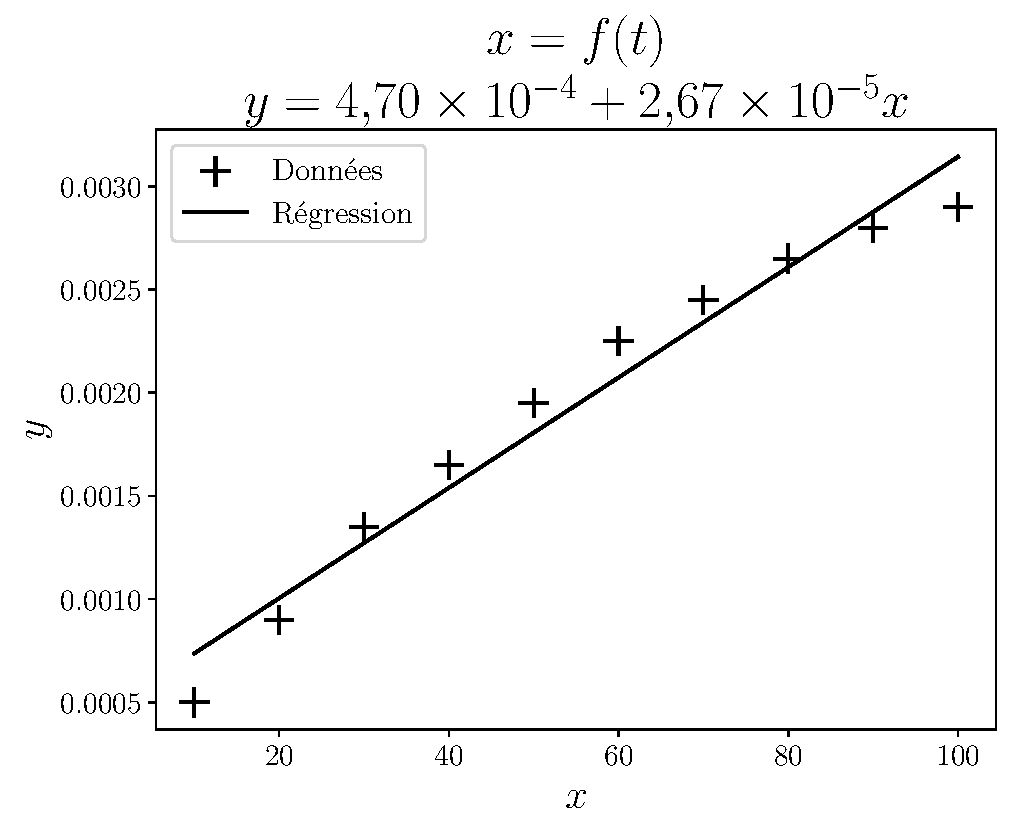
\includegraphics[width=\linewidth]{graph_1}}
		\subcaptionbox{$\ln (1-200x) = f(t)$}
		[.32\linewidth]
		{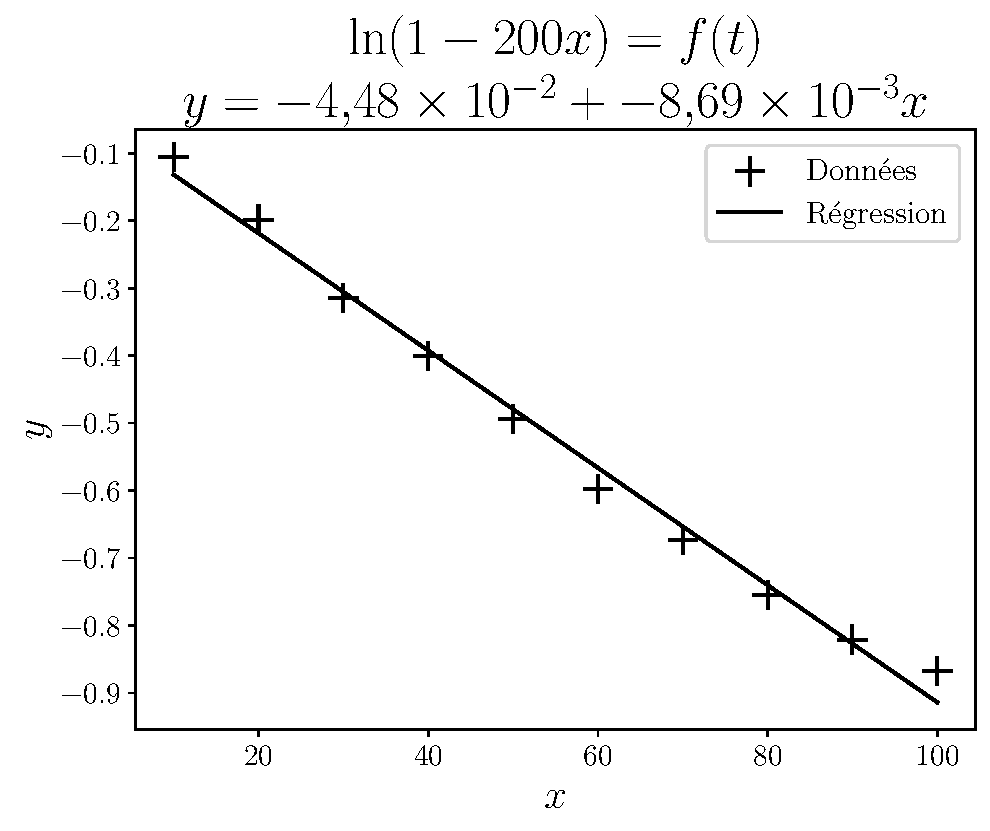
\includegraphics[width=\linewidth]{graph_2}}
		\subcaptionbox{$\frac{1}{0,01-2x} - 100 = f(t)$}
		[.32\linewidth]
		{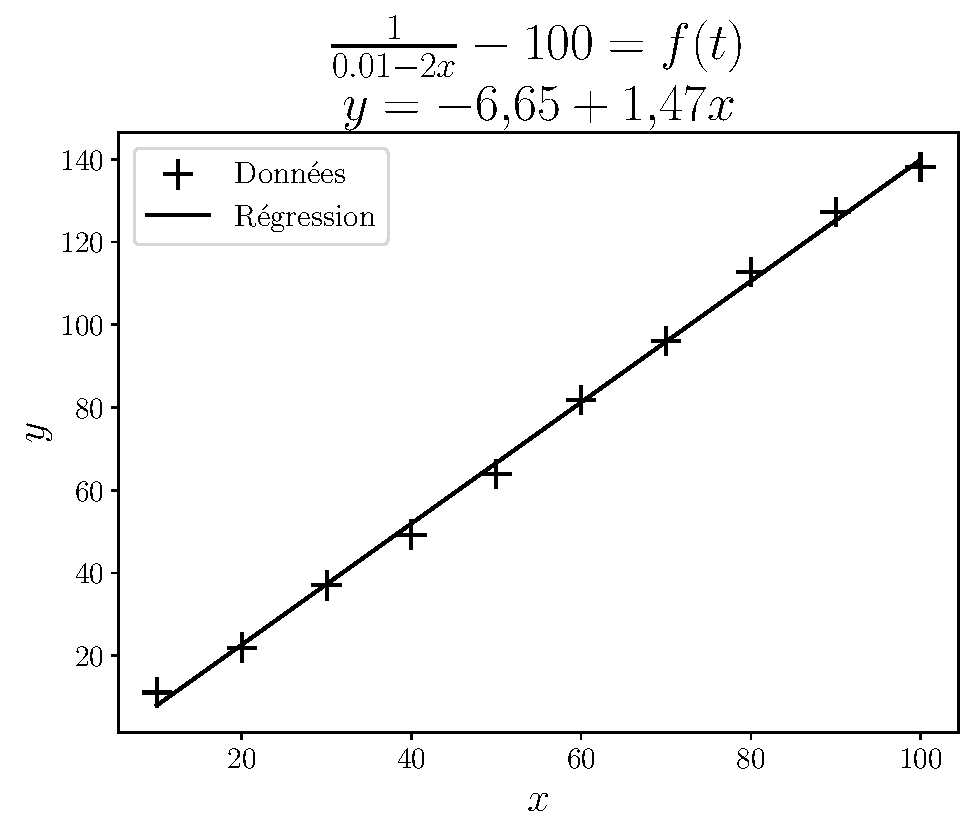
\includegraphics[width=\linewidth]{graph_3}}
		\caption{Graphiques.}
		\label{fig:graphs}
	\end{figure}
  % \begin{figure}[htbp!]
  %   \centering
  %   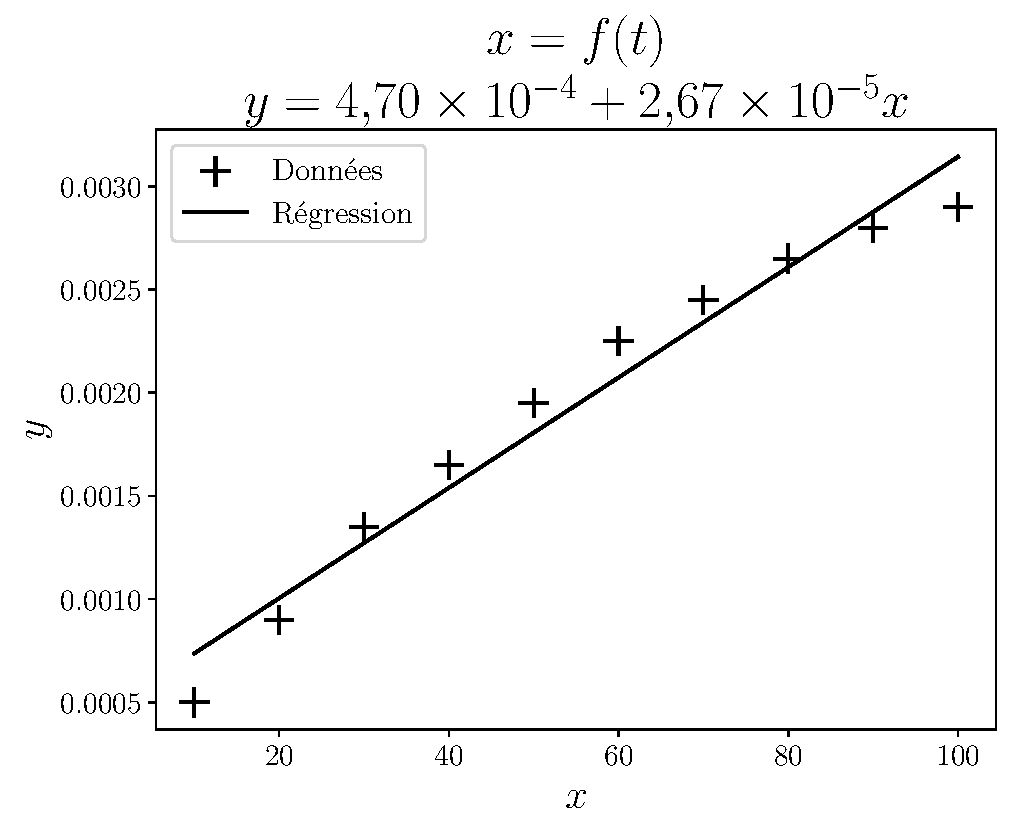
\includegraphics[width=.7\linewidth]{graph_1}
  %   \caption{Graphique 1~: $x=f(t)$}
  %   \label{fig:grph1}
  % \end{figure}
  %
  % \begin{figure}[htbp!]
  %   \centering
  %   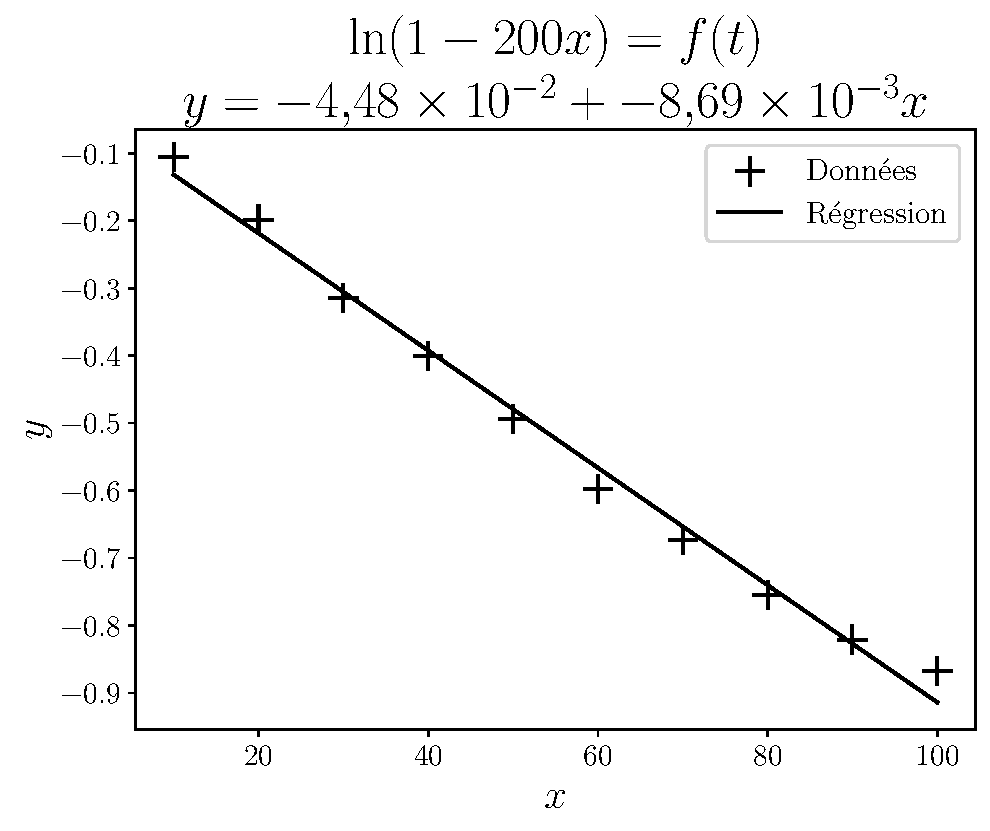
\includegraphics[width=.7\linewidth]{graph_2}
  %   \caption{Graphique 2~: $\ln (1-200x) = f(t)$}
  %   \label{fig:grph2}
  % \end{figure}
  %
  % \begin{figure}[htbp!]
  %   \centering
  %   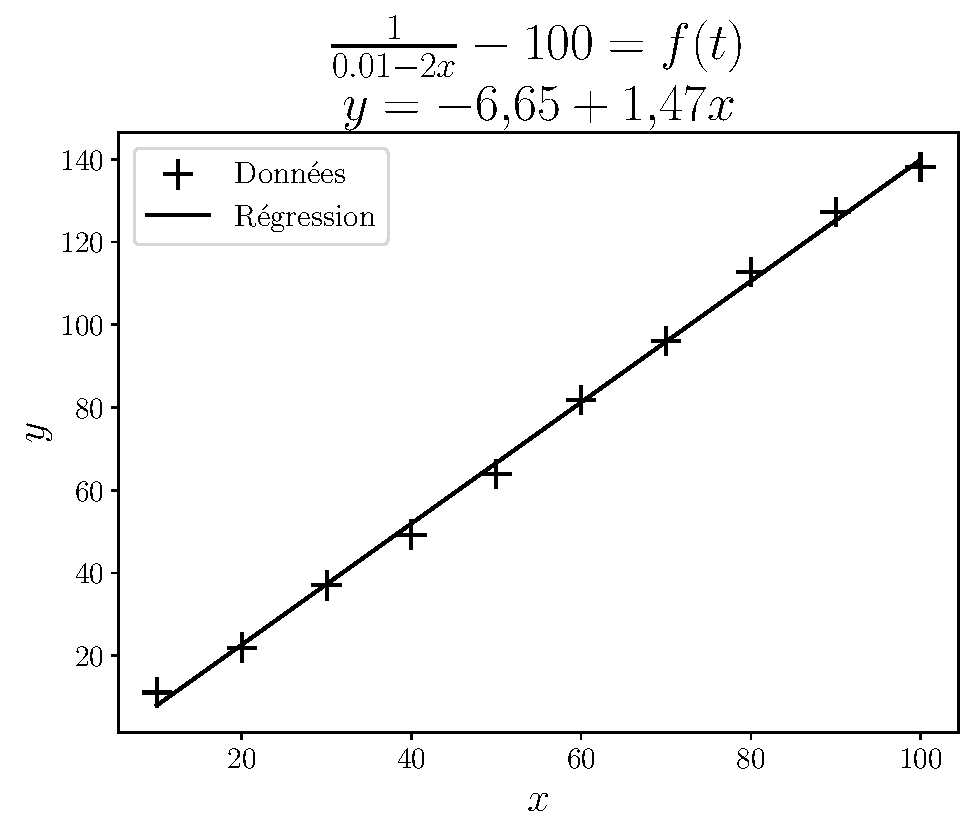
\includegraphics[width=.7\linewidth]{graph_3}
  %   \caption{Graphique 3~: $\frac{1}{0,01-2x} - 100 = f(t)$}
  %   \label{fig:grph3}
  % \end{figure}
}

\QR{%
  À l'aide d'un des graphes, déterminer l'ordre de la réaction et la constante
  de vitesse dont on précisera l'unité.
}{%
  La courbe qui ressemble le plus à une droite est la courbe 3~: les données
  sont réparties plus aléatoirement que la courbe 2 qui ressemble plus à une
  parabole. La première ne convient clairement pas.
  \par
  On en déduit que la réaction est le mieux modélisée par une réaction d'ordre
  2. La pente de la droite ajustée est $\SI{1,47}{\mol^{-1} s^{-1}} = 2k/V_0$.
  Puisque $V_0 = \SI{100e-3}{\litre}$, on en déduit que
  \[
    \boxed{k=\SI{7,35e-2}{\litre.\mol^{-1}\second^{-1}}}
  \]
}

\QR{%
  Que pensez-vous quant à la vitesse de dissolution des coraux dans l'océan~?
}{%
  La vitesse de dissolution des coraux est assez lente car elle est d'autant
  plus grande que la concentration en ions \ce{H+} est grande, c'est-à-dire que
  le pH est petit. Or, actuellement, le pH de l'océan est de l'ordre de $8,0$.
  Cependant, à cause des activités humaines, les océans s'acidifient en raison
  de la hausse de \ce{CO2} dissout dedans. Les coraux vont donc se dissoudre
  de plus en plus vite.
}
\end{document}
